
\section{RESULTS}

\subsection{Simulation variant 1 (selection method)}

Figure~\ref{selectionMethodBoxplot} presents a notched boxplot of the time to
convergence for the \textbf{selection with replacement} vs. \textbf{selection
without replacement} trials, with the \textsl{influence direction} variable
held constant at \textbf{neighbor influences node}. Clearly the \textbf{with
replacement} variant ($M$=7296, $SD$=5382) takes significantly longer (nearly
twice as long, in fact) to converge than does \textbf{without replacement}
($M$=4084, $SD$=3493), as a two-sided t-test for the difference of means
confirms (t(341)=7.080, p=$8\times 10^{-12}$).

\begin{figure}[ht]
  \centering
  \subfloat[Comparison of \textsl{selection method} levels, with \textsl{influence
direction} set to \textbf{neighbor influences node}.]{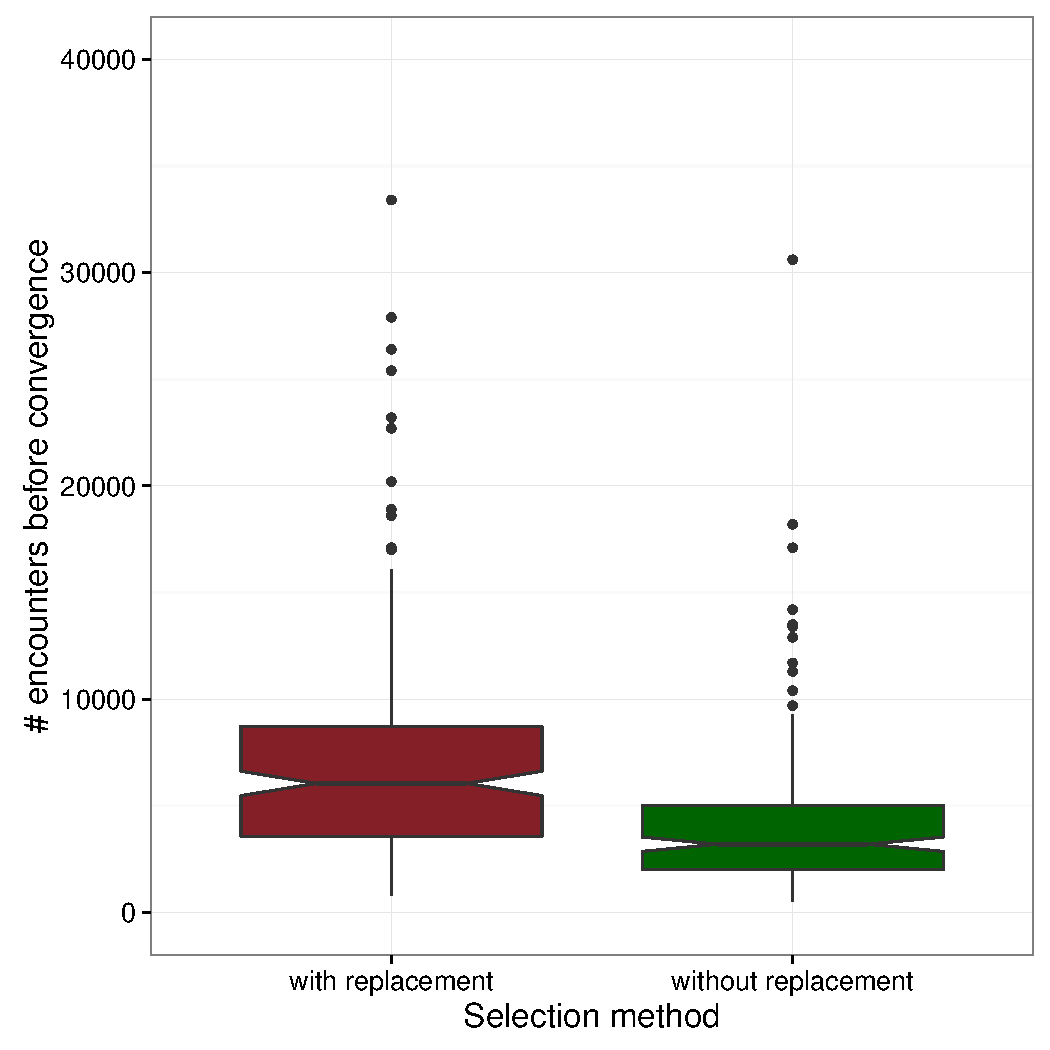
\includegraphics[width=0.4\textwidth]{selectionMethodBoxplot.pdf}\label{selectionMethodBoxplot}}
  \hfill
  \subfloat[Comparison of \textsl{influence direction} levels, with \textsl{selection
method} set to \textbf{without replacement}.]{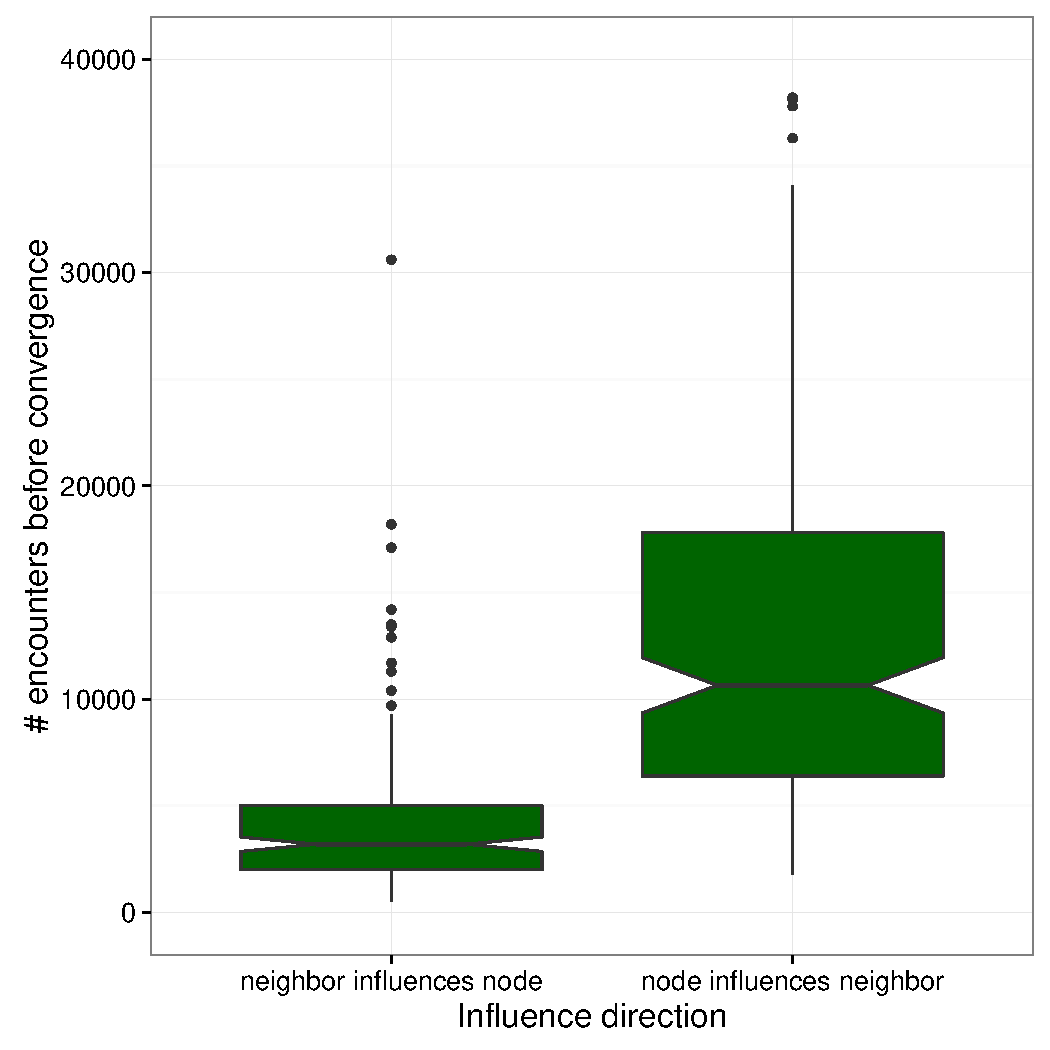
\includegraphics[width=0.4\textwidth]{influenceDirectionBoxplot.pdf}\label{influenceDirectionBoxplot}}
  \caption{Time to convergence of uniformity of opinion (N=400). (A few of the
largest outliers have been omitted for the sake of readability.)}
\end{figure}


The explanation for this difference would appear to be the following. If the
nodes to be influenced are selected \textit{with} replacement, then inevitably
some nodes will be relatively unaffected by their neighbors even as other
nodes have their opinions updated multiple times. Thus the permeation of the
to-be-dominant opinion throughout the system is uneven: the contagion reaches
and ``converts" some parts of the graph long before the ``starved" nodes are
influenced. Conversely, if chosen without replacement, every node in the graph
regularly has a chance to be influenced, which means no hold-outs can ``hide"
in the graph.

% This is confirmed (?) by counting how many encounters actually result in
% conversions.




\subsection{Simulation variant 2 (influence direction)}

An even greater difference in convergence time exists between the
\textbf{neighbor influences node} ($M$=4084, $SD$=3493) and \textbf{node
influences neighbor} ($M$=14417, $SD$=11492) variants, this time holding
\textsl{selection method} constant at \textbf{selection without replacement}
(see Figure~\ref{influenceDirectionBoxplot}.) A t-test for the difference
between these means yields t(235)=--12.16, p=$2\times 10^{-16}$).

Two explanations of this behavior suggest themselves. The first is a similar
``unevenness" argument that we offered for simulation variant 1: if every node
is regularly chosen to \textit{be} influenced, this should promote fairly
rapid convergence of the graph as a whole. But if every node is simply chosen
regularly \textit{to} influence, then there is nothing stopping some of the
nodes from receiving very infrequent influence. This, then, would lead to
longer convergence times.

A second, more subtle argument relates to the non-uniform degree distribution
of an Erdos-Renyi (or indeed, almost any) graph. Some nodes are connected to
many neighbors, while others are connected to very few. This means that while
under \textbf{neighbor influences node}, a low-degree node will be influenced
at the same rate as the others, if \textbf{node influences neighbor} is in
play, it has a very low probability of ever being influenced. For this to
happen, one of its very few neighbors would have to be chosen in an iteration
(a rare event), and then of all that neighbors' neighbors, the low-degree node
would have to be the ``lucky" one chosen. The necessity of both of these
unlikely occurrences happening together makes low-degree neighbors unwittingly
stubborn indeed (under \textbf{node influences neighbor}, which is perhaps
responsible for variant 2 having even larger convergence time differences than
variant 1.


\subsection{Variable interactions}

Finally, we point out a non-trivial interaction between the two factors. As
illustrated in Figure~\ref{interactionBoxplot}, the difference in convergence
times between the two \textsl{selection method}s is only significant under the
\textbf{neighbor influences node} level. A 2$\times$2 ANOVA for the entire
800-trial design revealed a main effect for \textsl{influence direction},
F(1)=186.00, p=$2\times 10^{-16}$, but no significant effect for
\textsl{selection method}, F(1)=1.26, p=$.261$. An interaction between the two
effects was significant, F(1)=20.42, p=$7\times 10^{-6}$.

\begin{figure}[ht]
\centering
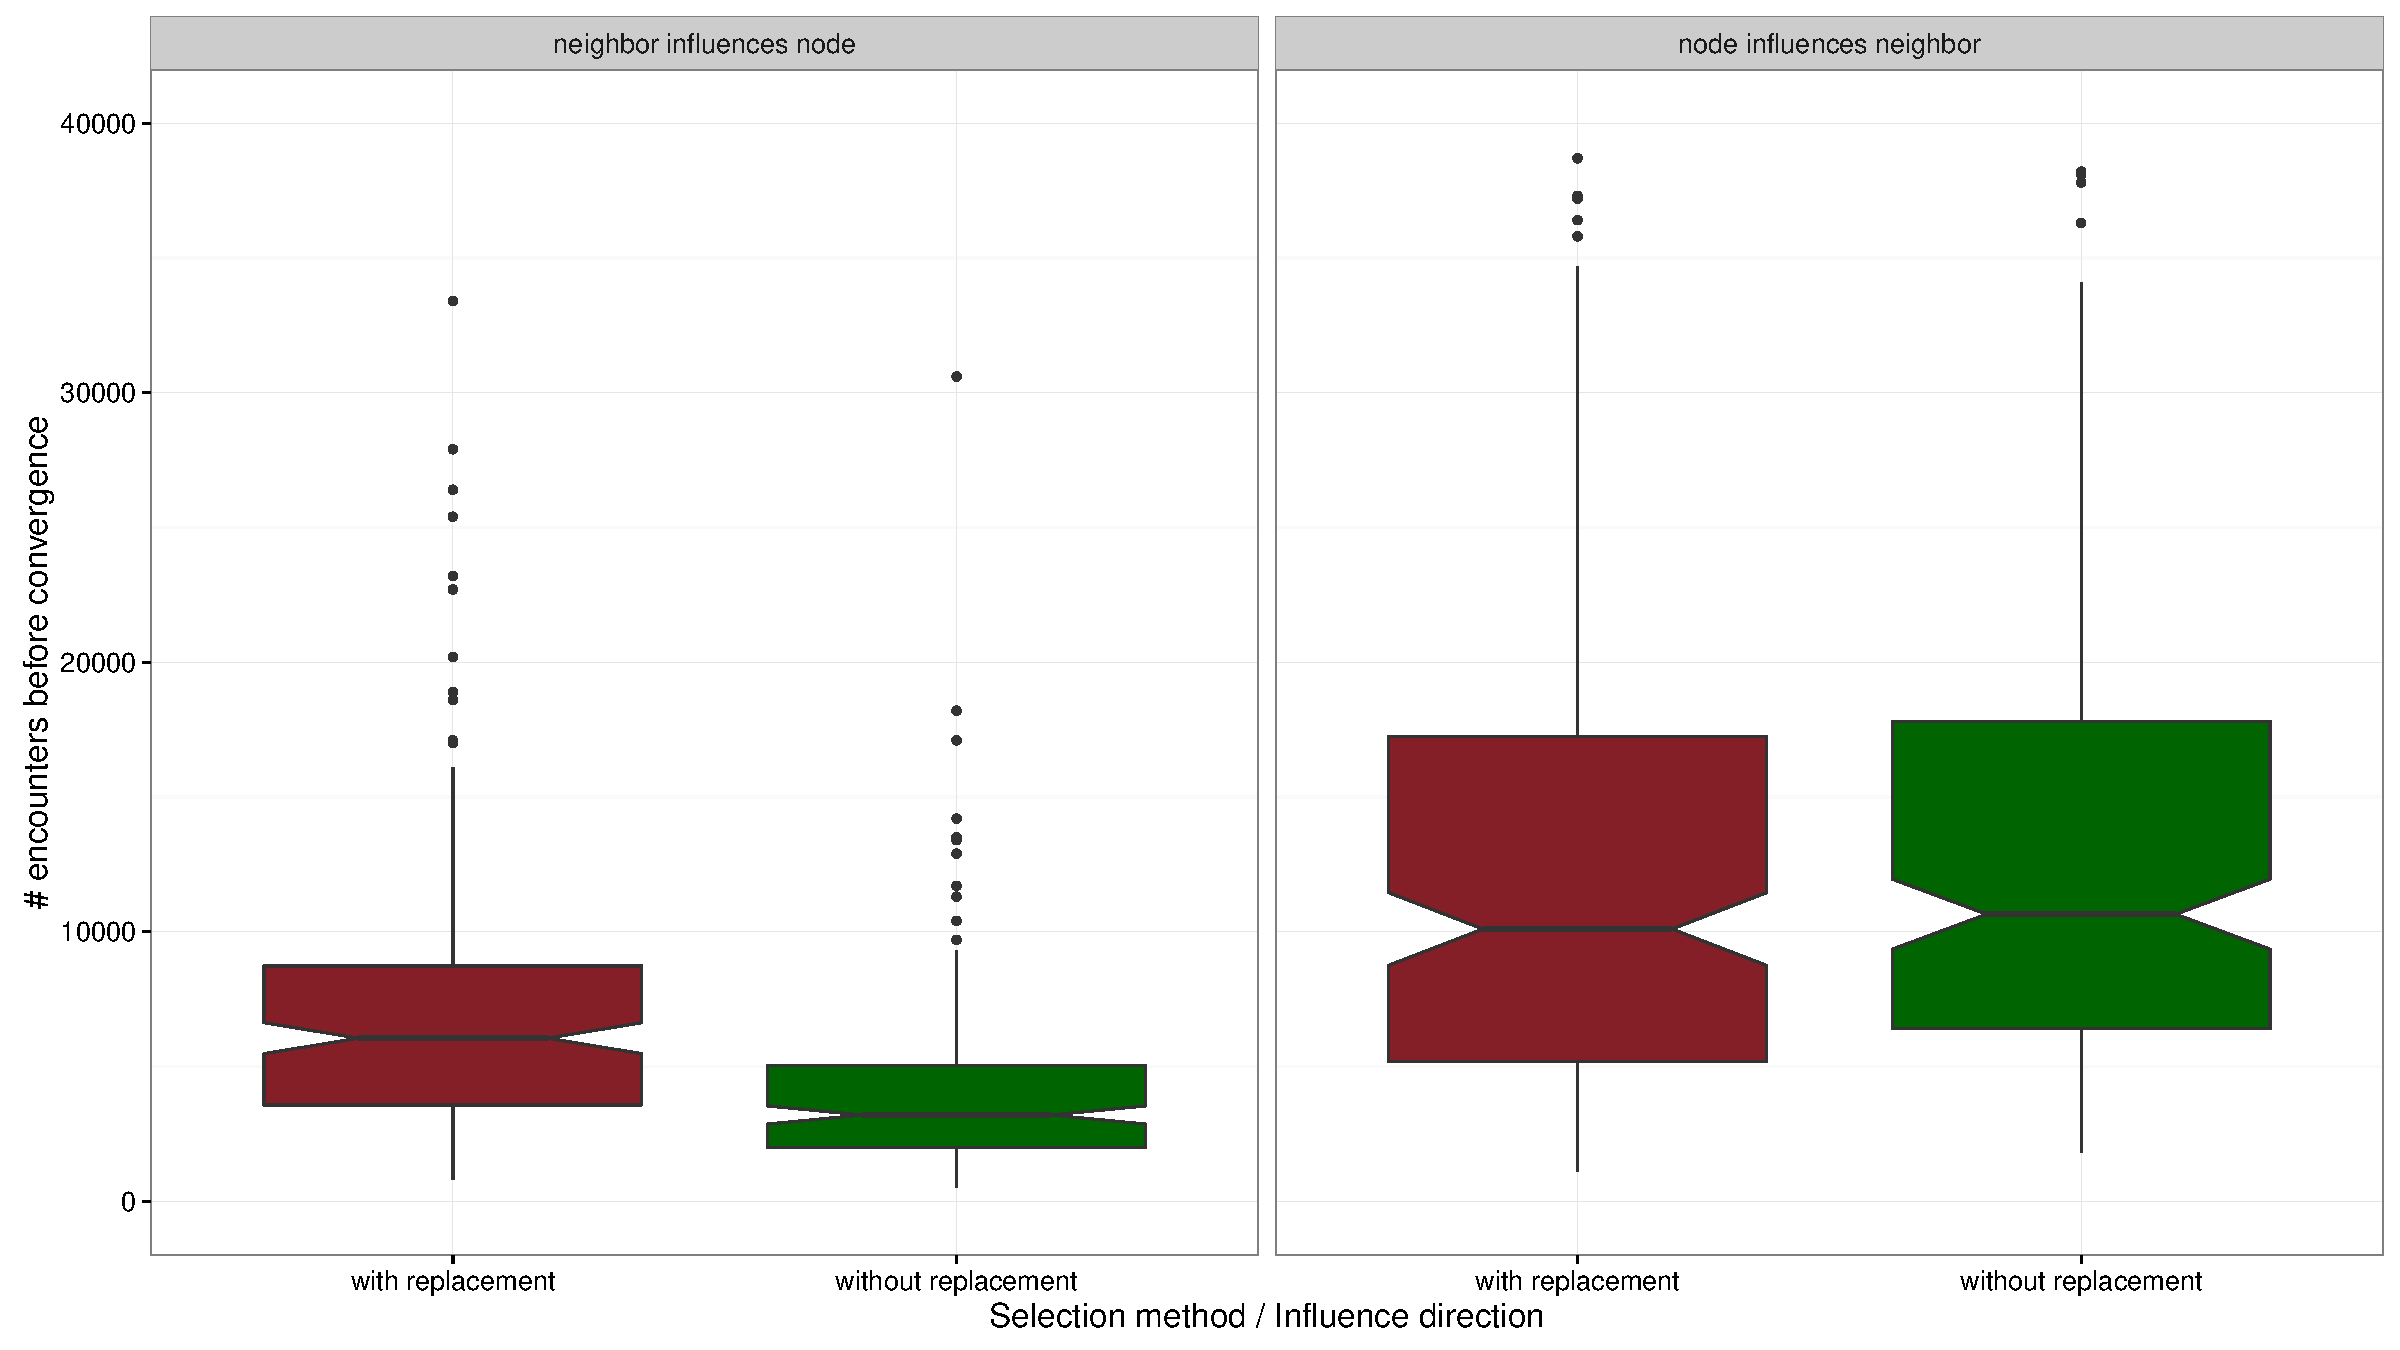
\includegraphics[width=0.9\textwidth]{interactionBoxplot.pdf} 
\caption{Full factorial design results for all four groups, illustrating
interaction between effects (N=800). (A few of the largest outliers have been
removed.)}
\label{interactionBoxplot}
\end{figure}

The reason for the interaction is fairly straightforward, stemming directly
from the analysis in the sections above. When \textbf{neighbor influences
node}, it matters very much whether all nodes are chosen on a regular basis,
since if some are not, they have no chance to change their opinion, causing an
impediment to convergence. If \textbf{node influences neighbor}, on the other
hand, the only thing at stake with the \textsl{selection method} choice is
which nodes get to do the most influencing. When some nodes are noticeably
less \textit{influential} than others, we can perhaps expect some impact on
convergence time (and even then, it's not clear in which direction), but we
will not experience a strong, consistent dampening effect as we will when some
nodes are noticeably less \textit{influenced} than others.

